%%%%%%%%%%%%%%%%%%%%%%%%%%%%%%%%%%%%%%%%%%%%%%%%%%%%%%%%%%%%%%%%%%%%%%%%%%%%%%%%
\chapter{Постановка задачи}
\label{chap:task}

В данной работе для анализа использовались обращения пользователей в техническую поддержку системы отслеживания ошибок YouTrack\footnote{http://jetbrains.ru/products/youtrack/}. Для взаимодействия с пользователями команда YouTrack использует Zendesk\footnote{https://www.zendesk.com}~--- систему учета и обработки пользовательских обращений.

\begin{figure}[tph!]
\centerline{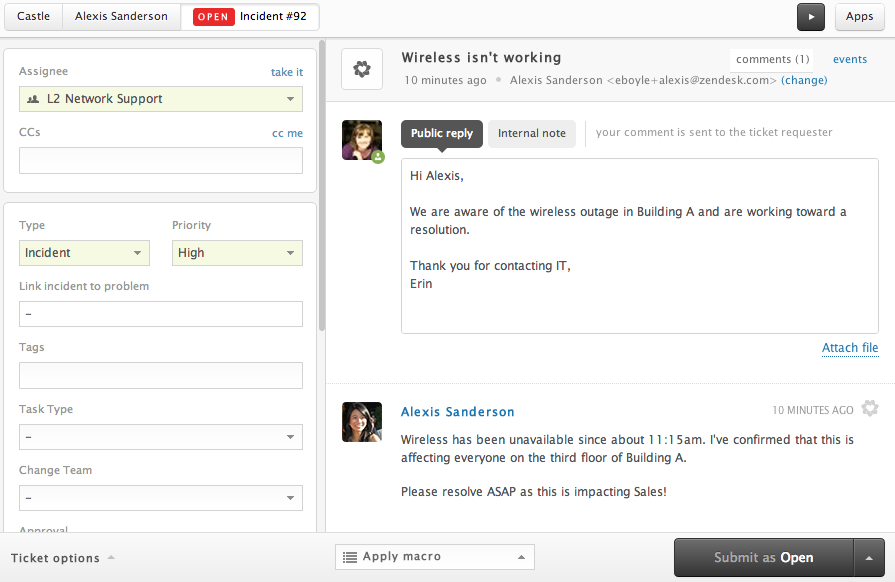
\includegraphics[width=11cm]{fig/zendesk2.png}}
    \caption{Пример обращения в системе Zendesk}
    \label{fig:zdesk_ticket}
\end{figure}

В Zendesk обращения могут поступать из различных каналов: электронная почта, социальные сети, форма для прямой отправки обращений и так далее. Обращения состоят из комментариев и, в общем случае, представляют собой диалог между клиентом и сотрудником технической поддержки. На рисунке~\ref{fig:zdesk_ticket} приведен пример обращения в системе Zendesk. Поскольку Zendesk агрегирует все поступающие  обращения, то мы не можем делать предположений о их разбиении по темам. То есть заранее неизвестно, какие из обращений относятся, например, к проблемам администрирования YouTrack, а какие~--- связаны с пользовательским интерфейсом.

Было проанализировано 6500 обращений за период с декабря 2015 года по сентябрь 2016 года. Стоит отметить, что на момент написания статьи работа еще не была завершена, однако промежуточные результаты показывают, что подход может быть применен для генерации ЧЗВ. Из предложенных эксперту ВОП 50\% было признано корректными по сравнению с 37\%, полученными в работе~\cite{original}.

%%%%%%%%%%%%%%%%%%%%%%%%%%%%%%%%%%%%%%%%%%%%%%%%%%%%%%%%%%%%%%%%%%%%%%%%%%%%%%%%
\section{Формулирвоание требований}
\label{sec:features}
%%%%%%%%%%%%%%%%%%%%%%%%%%%%%%%%%%%%%%%%%%%%%%%%%%%%%%%%%%%%%%%%%%%%%%%%%%%%%%%%
\blindtext
%%%%%%%%%%%%%%%%%%%%%%%%%%%%%%%%%%%%%%%%%%%%%%%%%%%%%%%%%%%%%%%%%%%%%%%%%%%%%%%%
\section{Решаемые задачи}
\label{sec:tasks}
%%%%%%%%%%%%%%%%%%%%%%%%%%%%%%%%%%%%%%%%%%%%%%%%%%%%%%%%%%%%%%%%%%%%%%%%%%%%%%%%
\blindtext
%%%%%%%%%%%%%%%%%%%%%%%%%%%%%%%%%%%%%%%%%%%%%%%%%%%%%%%%%%%%%%%%%%%%%%%%%%%%%%%%
\section{Вывод}
\label{sec:task_concl}
%%%%%%%%%%%%%%%%%%%%%%%%%%%%%%%%%%%%%%%%%%%%%%%%%%%%%%%%%%%%%%%%%%%%%%%%%%%%%%%%
\blindtext